It is not only for stack or heap elements which we need to store information
about their type. Sub-routines and object fields also has type information which
we need to keep track of, but the information is not the same. For instance, a
stack or heap element has types describing the type of its value. A sub-routing
will need have a type signature, describing the types of it's parameters, a name
and possible properties. Similarly an object field will have (TODO).

Therefore, we need to abstract our type information a level higher, letting us
better describe different types of types. Instead of storing the different data
different places, we will have a centralized table, containing all meta
information. This will be named the \term{meta table} and will need to be
dynamically sized to support reflection and generating new types at run-time.

All meta objects in the machine will have a tag defining which of type of
information it contains.
\begin{ccode}
enum meta_tag_e {
    TYPE,
    METADATA,
    FIELD,
};
typedef enum meta_tag_e meta_tag;

struct meta_base_s {
    meta_tag tag;
};
typedef struct meta_base_s meta;

struct meta_type_s {
    meta base;

    type *type;
};
typedef struct meta_type_s meta_type;
\end{ccode}
In the case of {\tt TYPE} it will be cast to the {\tt meta\_type} which allows
access to the {\tt type} referenced described below.

We will describe each type of meta information in turn.

\subsubsection{Types}
The executable file, containing the program to be run, defines a type table for
the custom types created by the program. Throughout the executable, these types
are referenced through the type's index in this table. This table is static, so
the machine can analyze how many types it contains. The types will be parsed
from the executable and added to the global meta table lazily. This reduces the
initial overhead of parsing the executable and avoids loading types that will
not be used during run-time.

The machine's built-in types are described by a type tag, implemented as an enum:

\begin{ccode}
enum type_tag_e {
    ACTIVATION_ELEMENT = 0,
    ANY                = 1,
    BOOL               = 2,
    INT8               = 3,
    UINT8              = 4,
    ...
};
typedef enum type_tag_e type_tag;
\end{ccode}

The enum's integer value is used to describe its index in the meta table. There
will always only be a single instance of each type, so two equal types can never
be referenced by two different pointers, similar to how DWARF types are stored
(as described in Section~\ref{sec:design:types:dwarf}). This invariant lets the
machine check type equality simply by comparing the type pointers.

More specifically, all types in the machine are stored internally through
structs. Simple types implement the {\tt type\_base} struct, which is extended
in composite types. For instance, a reference is represented as:

\begin{ccode}
struct type_base_s {
    type_tag tag;
    int size;
};
typedef struct type_base_s type;

struct type_ref_s {
    type base;
    type *ref_type;
};
typedef struct type_ref_s type_ref;
\end{ccode}

All types are always passed around in the machine through the {\tt type}
name. If the type is for instance a reference, i.e.~implementing the {\tt
  type\_ref}, it is cast so its reference specific attributes can be
referenced. The type of type is checked through the tag, defined in {\tt
  type\_base}. Another important entry in the type structure is the size
attribute. This is essential, as it tells the machine how much memory is needed
to store a value of that type on either the stack or heap.

Types from the executable are mapped from its index in the binary type table to
the machines meta table. As the executable meta table is of static size, this
will be a simple integer array, mapping binary meta index to the machines actual
meta entry pointer. The meta entries will be parsed lazily, i.e. the first time
the program tries to look-up a meta entry through its index in the binary meta
table, it is parsed and stored in the machine's meta table.

The machines internal meta table is implemented through a hash map, where each
meta entry can be looked up through it's hashed value. Having implemented the
meta table as a hash table lets us lookup entries in constant time, removing
overhead from iterating. The only requirement of the hashing function is that it
makes unique hashed for meta entry that are equal. This is currently done with a
simple implementation of Bob Jenkins' One-at-a-time
hash~\footnote{\url{https://en.wikipedia.org/wiki/Jenkins_hash_function\#one-at-a-time}}. We
have chosen this hash function due to relatively good speed and uniqueness,
compared to more complex hashing functions. Bob Jenkins himself has written
article comparing several similar functions and their running speed, which we
used as reference~\cite{jenkins}. To get a reference to a built-in type, one can
look-it up through a look-up function, which takes a meta hash. This can be done
through a strict function which thrown an exception if the hash is not found, or
a lazy function which will generate the new meta entry if not found. This is
especially useful for looking up types, not guaranteed to already be found in
the meta table.

%TODO: this should be under instructions?
When trying to box a stack element trough the {\tt box} instruction, the top
element is popped off the stack and stored on the heap. An element with a
reference to the heap object is in turn pushed to the stack. The type of the new
element will be a {\tt Reference<t>} type, where {\tt t} is the type of the
stack element which was boxed. If this type is not found in the meta table
already it is generated at run-time.

% TODO: removed since it's discussed under type lattice. vale?
% Most types can be converted, with some exceptions (TODO signature type). If a
% value is converted to a type with smaller size, for instance an {\tt Int32} to
% {\tt Int8}, the value is truncated (TODO exception)?

% TODO: move along?
% All types are garbage collected. This means, when a type is no longer used by
% the program, it's memory is freed. (TODO)

% TODO how to structure this?

\subsubsection{Composite Types}

Composite types are used to describe heap objects, stack objects and
scopes. They consist of a name and a set of members which are implemented as an
array of pointers to meta data entries which must be either fields or
sub-routines. Members are looked up during run-time by use of a meta data entry
that describes the field or sub-routine. The idea is that a heap object's (or
stack object's or scope's) associated type includes the members, so modification
of the heap objects actual data is possible by providing the definition of the
desired member that maps to a field or sub-routine. See
Section~\ref{implementation:meta:fields}
and~\ref{implementation:meta:sub-routines} for details of how fields and
sub-routines are used to modify a heap object.

The list of members is dynamic meaning that members can be added
or removed during run-time. This is a very useful feature for dynamic languages
in which it is a common feature to be able to modify the list of properties on
an object during run-time. The current implementation however does not support
this, but would likely be implemented via run-time library functions.

\subsubsection{Floating Point Value Types}

When handling floating point precision numbers we will, as aforementioned, use
the IEEE 754 standard~\cite{ieee754}. This is a technical standard defining the
arithmetic format, i.e.~the finite range and special values, rounding rules,
operations, exception handling and interchange formats. Its values include
finite numbers (within a certain maximum or minimum, depending on the size), two
infinities (plus and minus) and a NaN (not a number).

A floating point number is always represented by a sign, a fraction (also called
significant or mantissa), and an exponent. A can have multiple alternative
representations, for instance $1.10 \cdot 10^2$ can also be written as
$11.00 \cdot 10^1$. This though, should not have any effect on the result of
arithmetic operations. When storing the number in memory, one bit is used for
sign and the rest for exponent and fraction, depending on the size. The most
common the is single and double precision, which is respectively 4 and 8 bytes
in size. Their binary representation is called {\tt binary32} and {\tt
  binary64}.

\begin{figure}[H]
  \centering
  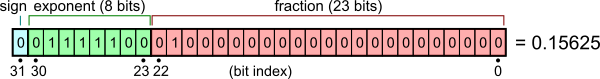
\includegraphics[scale=0.7]{images/ieee32.png}
  \caption[Caption for LOF]{IEEE-754 binary32 encoding~\footnotemark}
\end{figure}
\footnotetext{\url{https://en.wikipedia.org/wiki/Single-precision_floating-point_format}}

When parsing a {\tt binary32} we start by taking all the correct bits out into
separate numbers. We can then apply the following formula to get its decimal
value.

\begin{equation}
  value = (-1)^{sign} \cdot (1 + \sum^{23}_{i=1} b_{23-i}2^{-i}) \cdot 2^{e - 127}
\end{equation}

% type lattice

When performing arithmetic instruction on numbers, the machine enforces strong
typing and will therefore throw an exception if the operands is not of the same
type. This is to avoid common pitfalls, such as not handling overflow of
numbers, but also when doing arithmetic operations of two different types of
numbers. If a program, for instance, divides a floating point precision number
by an integer number, will the result be an floating point or integer? The only
case the machine it self needs to make a choice is with stack elements of type
{\tt AnyType}. Instead of having a long list of what do do in every case of all
types, the choice will be defined by a type lattice. This type lattice will
control what type the result is of a given operation between two numbers of
different types.

All binary arithmetic operations follow the same type lattice (TODO:
correct?). The type lattice has the following set of rules matching which
operand that is to be converted, where the resulting conversion is also the type
of the result.
\begin{itemize}
  \item If both operands is of the same type, nothing needs to be done.
  \item Otherwise, if either operand is a double floating-point precision
    number, the other operand is converted to a double also.
  \item Otherwise, if either operand is a single floating-point precision
    number, the other operand is converted to a float also.
  \item Otherwise, if either operand is of different signs, i.e. one is unsigned
    and the other is signed, the signed operand is converted to the an signed
    integer of the largest size of the two operands.
  \item Otherwise, the operands is of integer types of the same sign, where we
    return the largest of the two.
\end{itemize}

If none of the rules apply it will mean that at least one of the given operands
is of a type not supporting arithmetic operations. In this case, an exception
will be thrown.

If a type is converted to a type of smaller size, the value it truncated and
will have the chance of overflowing, changing the value of the number. The {\tt
  noOverflow} prefix defines if an exception should be thrown if overflow
occurs. There are though, separate instruction for saturated arithmetic
operations, where overflow is handled by saturating the number of the given
type. For instance, converting {\tt 0xFFFF} of type {\tt Int16} to {\tt Int8}
will become {\tt 0xFF}.


\subsubsection{Fields}
\label{implementation:meta:fields}
% meta data
% described by composite member
% has name, type, offset

Fields are also a type of meta data, describing a member of a {\tt Composite}
type, in the form of field definition. It is important to note that fields are
not types them selves, like {\tt Composite} is, but a meta element describing a
field definition. Consequently, a field definition has a type element describing
the type the fields' content.

The internal data representation of a field definition, is as all other meta
types, an extension of the {\tt meta\_base} struct, giving it a type of meta, in
the form of a tag, and a unique hash. The field definition struct, {\tt
  meat\_field} extends this by adding a name, which is a index into the string
table, an integer offset, which is the distance where its value is stores from
the beginner of the heap object, and lastly a type describing its content. I
addition to these it a has an arbitrary number of properties and versions, which
is not yet implemented. The version element is to support dynamic languages
(TODO) which can be extended or monkey patched, as Rubyists like to call
it. Therefore, a number of similar fields can exist in memory, which are
distinguished by version. % TODO
\begin{ccode} % TODO: update
struct meta_field_s {
    meta base;

    str_index name;
    int offset;
    type *type;

    /* missing: props, versions */
};
\end{ccode}

A field can be defined with set of properties, modifying its
functionality. Such properties are {\em abstract}, where the field is not
actually initialized, only declared. This is useful for languages with
interfaces or abstract methods, akin to Java's abstract classes and methods
where another class can extends the abstract class, implementing its already
defined fields and methods.

Another property is {\em final}, where the the specific content of the field
cannot be changes. If the content is a reference, for instance, the reference
will always be the same, but the value of reference may still be mutated (TODO:
correct?).

The last property is {\em strict layout}, where the value of the field is
guaranteed to be placed directly preceding to the field definition on the
heap. This enabled the compiler to the {\tt offset} element to reference the
content of the field. This is though considered unsafe, and thus the instruction
must be prefixed with the {\tt unsafe} flag.

%%% Local Variables:
%%% mode: latex
%%% TeX-master: "../report"
%%% End:
